\documentclass[border=4pt]{standalone}

% --- packages (mirror these in container.meta.json "requires") ---
\usepackage{tikz}

% --- palette (canonical source: reference/color-palettes/color-palettes.md; light variant) ---
\definecolor{otblue}{HTML}{0072B2}
\definecolor{otorange}{HTML}{E69F00}
\definecolor{otteal}{HTML}{009E73}
\definecolor{otpurple}{HTML}{CC79A7}
\definecolor{otgray}{HTML}{5A5A5A}

\begin{document}
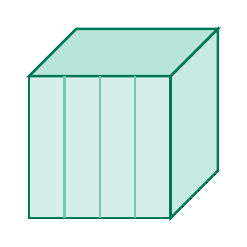
\begin{tikzpicture}[line width=0.9pt]
  % front face
  \filldraw[draw=otteal!75!black, fill=otteal!16] (0,0) rectangle (1.8,1.8);
  % top face
  \filldraw[draw=otteal!75!black, fill=otteal!28] (0,1.8) -- (0.6,2.4) -- (2.4,2.4) -- (1.8,1.8) -- cycle;
  % right face
  \filldraw[draw=otteal!75!black, fill=otteal!22] (1.8,0) -- (2.4,0.6) -- (2.4,2.4) -- (1.8,1.8) -- cycle;
  % container slats on the front
  \foreach \x in {0.45,0.9,1.35}{ \draw[otteal!55] (\x,0) -- (\x,1.8); }
\end{tikzpicture}
\end{document}
